\documentclass[qual, classic, a4paper]{ufbathesis}
%\usepackage[hidelinks=true,colorlinks=false]{hyperref}
\usepackage[utf8]{inputenc}
\usepackage[colorinlistoftodos,prependcaption,textsize=tiny]{todonotes}
\usepackage{float}
\usepackage{microtype}
\usepackage{ dsfont }
%\usepackage{xcolor}
\usepackage{indentfirst}
%%\usepackage[T1]{fontenc}
\usepackage[alf]{abntex2cite}
\usepackage{acronym}
\usepackage{tikz}
\usepackage{soul}
\usepackage[portuguesekw, portuguese, ruled, linesnumbered]{algorithm2e}
\usepackage{amssymb,amsmath,amsthm}

%\usepackage[toc,symbols]{glossaries}

%\usepackage[toc, nonumberlist, style=altlist]{glossaries}
%\newglossary[slg]{symbolslist}{syi}{syg}{Lista de S\'imbolos}

%\usepackage[symbols,nogroupskip]{glossaries-extra}

%\onehalfspacing
%\newtheorem{theorem}{Theorem}
%\newtheorem{hipotese}{Hipótese}

%%Siglas
\acrodef{HHC}{\textit{Home Health Care}}
\acrodef{HHCP}{\textit{Home Health Care Problem}}
\acrodef{HHCSP}{\textit{Home Health Care Scheduling Problem}}

\acrodef{HHCRSP}{\textit{Home Health Care Routing and Scheduling Problem}}
\acrodef{PERE}{\textit{Problema de Escalonamento e Roteamento de Enfermeiras}}


\acrodef{NSP}{\textit{Nurse Scheduling Problem}}
\acrodef{PEE}{\textit{Problema de Escalonamento de Enfermeiras}}

\acrodef{NRP}{\textit{Nurse Routing Problem}}
\acrodef{PRE}{\textit{Problema de Roteamento de Enfermeira}}

\acrodef{CSP}{\textit{Crew Scheduling Problem}}
\acrodef{PAET}{Problema de Alocação de Equipe técnica}


\acrodef{TSP}{\textit{Traveling Salesman Problem}}
\acrodef{PCV}{Problema do Caixeiro Viajante}

\acrodef{PMCV}{Problema Múltiplo do Caixeiro Viajante}

\acrodef{VRP}{\textit{Vehicle Routing Problem}}
\acrodef{PRV}{\textit{Problema de Roteamento de Veículo}}

\acrodef{VRPTW}{\textit{Vehicle Routing Problem With Time Window}}
\acrodef{PRVJT}{Problema de Roteamento de Veículo com Janela de Tempo}

\acrodef{TSPTW}{\textit{Traveling Salesman Problem With Time Window}}
\acrodef{PCVJT}{Problema do Caixeiro Viajante com Janela de Tempo}

\acrodef{GRASP}{\textit{Greedy Randomized Adaptative Search Procedure}}
\acrodef{AICS}{\textit{Adaptative Iterated Construction Search}}
\acrodef{DLS}{\textit{Dynamic Local Search}}
\acrodef{ILS}{\textit{Iterated Local Search}}
\acrodef{VNS}{\textit{Variable Neighborhood Search}}
\acrodef{VDS}{\textit{Variable Depth Search}}

\acrodef{FESFSUS}{Fundação Estatal Saúde da Família}
\acrodef{SAD}{Serviço de Atenção Domiciliar}

\acrodef{IEEE Xplore}{Instituto de Engenheiros Eletricistas e Eletrônicos}
\acrodef{ACM}{ACM digital Library}
\acrodef{NHS}{National Health Service}

%% Identificacao:

% Universidade
\university{UNIVERSIDADE FEDERAL DA BAHIA}

% Endereco (cidade)
% e.g. \address{Campinas}
\address{Salvador}

% Instituto ou Centro Academico
% e.g. \institute{Centro de Ciencias Exatas e da Natureza}
% Comente se nao se aplicar
\institute{INSTITUTO DE MATEM\'{A}TICA}

% Nome da biblioteca - usado na ficha catalografica
% default: nome da biblioteca do Instituto de Matematica
%\library{BIBLIOTECA REITOR MACÊDO COSTA}

% Programa de pos-graduacao
% e.g. \program{Pos-graduacao em Ciencia da Computacao}
\program{Programa de Pós-Graduação em Ciência da Computação}

% ?rea de titulacao
\majorfield{CIÊNCIA DA COMPUTAÇÃO}

% Titulo da dissertacao/tese
% e.g. \title{Sobre a conjectura $P=NP$}
\title{HEURÍSTICAS PARA O PROBLEMA DE  ESCALONAMENTO E ROTEAMENTO DE EQUIPES DO SERVIÇO DE ATEN\c{C}\~AO DOMICILIAR}

% Data da defesa
% e.g. \date{19 de fevereiro de 2003}
\date{NOVEMBRO DE 2017}

% Autor
% e.g. \author{Jose da Silva}
\author{JÚLIA MADALENA MIRANDA CAMPOS}

% Orientador(a)
% Opcao: [f] - para orientador do sexo feminino
%\adviser[f]{Prof. Dr. TIAGO DE OLIVEIRA JANUARIO}
\adviser{TIAGO DE OLIVEIRA JANUARIO}

% Orientador(a)
% Opcao: [f] - para orientador do sexo feminino
% e.g. \coadviser{Prof. Dr. Pedro Pedreira}
% Comente se nao se aplicar
%\coadviser{NOME DO(DA) CO-ORIENTADOR(A)}

%% Inicio do documento
\begin{document}
% USAR ENQUANTO NAO ESTIVER NA VERSAO FINAL


% Folha de rosto
\frontpage

%%
%% Parte pre-textual
%%
\frontmatter

%\pgcomppresentationpage
% Se seu trabalho for uma tese de doutorado do PGCOMP, use a linha acima
%\pgcomppresentationpage
% Se seu trabalho for uma disserta??o de mestrado do PGCOMP, use a linha acima
% acima e use \presentationpage
\presentationpage
% Se for qualificacao, use \presentationpage

% Ficha catalogrofica
\authorcitationname{Campos, J.} 
\advisercitationname{Januario, T.}

\catalogtype{QUALIFICA\c{C}\~{A}O DE MESTRADO} 


% Dedicatoria
% Comente para ocultar
%\begin{dedicatory}
%DIGITE A DEDICATORIA AQUI
%\end{dedicatory}

% Agradecimentos
% Se preferir, crie um arquivo ?? parte e o inclua via \include{}

\acknowledgements
A todos que de alguma forma ajudaram.

% Epigrafe
% Comente para ocultar
% e.g.
 \begin{epigraph}[]{Lews Carroll}
  Se vo\c{c}\^{e} n\~{a}o sabe pra onde quer ir, qualquer caminho serve.
 \end{epigraph}

% Resumo em Portugues
% Se preferir, crie um arquivo separado e o inclua via \include{}
%\resumo
%DIGITE O RESUMO AQUI
%%%%%%%%%%%%%%%%%%%%%
% Resumo em Português
%%%%%%%%%%%%%%%%%%%%%

\resumo
O Serviço de Atenção Domiciliar, caracteriza-se como uma modalidade de atenção à saúde composta por um conjunto de ações de prevenção, reabilitação e tratamento de doenças, prestadas em domicílio. Esse serviço tem se tornado cada vez mais presente como ação de saúde complementar ou substituto à internação hospitalar, pois oferece uma nova modalidade de atendimento às pessoas com quadro clinico estável que necessitam de cuidados. O roteamento e escalonamento da equipe de internação domiciliar é realizado de forma manual em diversos países, inclusive no Brasil, tornando o processo ineficiente e muitas vezes gerando resultados insatisfatórios. Estima-se que o profissional de atendimento domiciliar passam entre 18\% a 26\% do tempo de trabalho dentro do veículo realizando translados entre os pontos de atendimento. Na literatura, o \textit{Home Health Care Routing Scheduling Problem} (HHCRSP) tem como objetivo construir de forma integrada o roteamento dos veículos da equipe de atendimento domiciliar, assim como, o escalonamento das equipes que serão trasportadas em cada veículo, para que seja possível percorrer todos os locais de visita e atender a um conjunto de pacientes de forma eficiente. Este trabalho tem como objetivo investigar o HHCP e desenvolver uma solução heurística para aumentar o número de atendimentos da equipe de atenção domiciliar, tendo como estudo de caso a Fundação Estatal de Saúde da Família em Salvador.
% Palavras-chave do resumo em Portugues
\begin{keywords}
Escalonamento de Equipes, Roteamento de Veículos, Serviço de Atenção Domiciliar, Heurísticas, Pesquisa Operacional
\end{keywords}

%%%%%%%%%%%%%%%%%%%
% Resumo em Ingles
%%%%%%%%%%%%%%%%%%%

\abstract
The Home Care Service is characterized as a modality of health care composed of a set of actions for prevention, rehabilitation and treatment of diseases, provided at home. This service has become increasingly present as a complementary health action or substitute for hospital admission, as it offers a new modality of care for people with stable clinical conditions that need care. The routing and scheduling of the home hospitalization team is carried out manually in several countries, including Brazil, making the process inefficient and often generating unsatisfactory results. It is estimated that the home care professional spend between 18 \% to 26 \% of the working time inside the vehicle doing transfers between the service points. In the literature, the Home Health Care Routing Scheduling Problem (HHCRSP) aims to build in an integrated way the routing of the vehicles of the home care team, as well as the scheduling of the teams that will be transported in each vehicle, so that it is possible to cover all the places of visit and to attend a set of patients efficiently. This work aims to investigate the HHCP and develop a heuristic solution to increase the number of home care staff, with the State Foundation for Family Health in Salvador as a case study.
% Palavras-chave do resumo em Ingles
\begin{keywords}
Crew Scheduling, Vehicle Routing Problem, Home Health Care, Heuristics, Operational Research.
\end{keywords}


% Palavras-chave do resumo em Portugues
% \begin{keywords}
% DIGITE AS PALAVRAS-CHAVE AQUI
% \end{keywords}

% Resumo em Ingles
% Se preferir, crie um arquivo separado e o inclua via \include{}
%\abstract
% Palavras-chave do resumo em Ingles
% \begin{keywords}
% DIGITE AS PALAVRAS-CHAVE AQUI
% \end{keywords}

% Sumario
% Comente para ocultar
%\tableofcontents

% Lista de figuras
% Comente para ocultar
\listoffigures

% Lista de tabelas
% Comente para ocultar
\listoftables

%%
%% Parte textual
%%
\mainmatter
%\linespread{4}

%capitulos

%%%%%%%%%%%%%%%%%%%
% Sumario / Indice
%%%%%%%%%%%%%%%%%%%

% Comente para ocultar
\tableofcontents

%estilo de numeracao
\pagenumbering{arabic}

% Lista de figuras
% Comente para ocultar
%\listoffigures

% Lista de tabelas
% Comente para ocultar
%\listoftables

%% Parte textual
%\mainmatter



\xchapter{Introdução}{ }

O \ac{SAD}, caracteriza-se como uma modalidade de atenção à saúde composta por um conjunto de ações de prevenção, de reabilitação e de tratamento de doenças prestadas em domicílio.
Esse serviço tem se tornado cada vez mais presente de forma a complementar ou substituir a internação hospitalar, pois oferece uma nova forma de atendimento às pessoas com quadro clinico estável que necessitam de cuidados.
Essa modalidade de atendimento permite maior comodidade aos pacientes, aumentando o conforto e facilitando o apoio familiar, além de reduzir os riscos de contaminação hospitalar e a lotação nos hospitais \cite{Kergosien:2009}.
Por outro lado, o \ac{SAD} também possui algum desafios, tais como: a necessidade do deslocamento do profissional de saúde, o planejamento da escada de trabalho dos profissionais de saúde envolvidos, o aumento de custos para a família, nos casos da necessidade de manter equipamentos elétricos ligados, e a eventual estadia do cuidador ou enfermeiro.%\cite{portaL:2017}.   

Na busca da melhor qualidade de vida da população e na redução de custos hospitalares, o \ac{SAD} tem sido bastante incentivado em diversos países. 
No Brasil, esse serviço teve início na década de 1960, porém seu funcionamento foi regulamentado pelo Sistema Único de Saúde (SUS) na década de 90, a partir da lei n. 8.080, de 19 de Setembro de 1990 \cite{Silva:2010}, chegando a Salvador em 2012, através da \ac{FESFSUS}. 

A \ac{FESFSUS} é um órgão público, sem fins lucrativos, que atua em 69 municípios do Estado da Bahia desde a Lei Complementar Estadual n. 29, de 21/12/2007, tendo iniciado suas atividades em 2009, começando a atuar na Bahia a partir de 16 de Abril de 2012. A fundação possui como uma das suas atribuições fornecer atenção domiciliar, de forma gratuita para os moradores da cidade de Salvador e regiões metropolitanas. Atualmente existem 9 bases e 135 pacientes internados em domicílio, e uma equipe de profissionais composta por: dois médicos, um enfermeiro, quatro técnicos de enfermagem, e um fisioterapeuta, contando também com profissionais de apoio, sendo eles: um assistente social, um nutricionista e um fonoaudiólogo.

A \ac{FESFSUS} fornece serviço de atenção domiciliar a pacientes com médio ou alto grau de complexidade, como por exemplo: pacientes com sequelas de acidente vascular cerebral, cardiopatas, portadores de paralisia infantil, politraumatizados, perfurados por armas de fogo e pacientes em tratamento oncológico.

Apesar do \ac{SAD} já existir há bastante tempo e em diversos países, ainda existem alguns desafios, tais como, o planejamento do escalonamento das equipes de atenção domiciliar e do roteamento dos veículos destinados a conduzir as equipes que irão realizar os atendimentos.

O Problema de Escalonamento e Roteamento de Equipes do Serviço de Atenção Domiciliar, conhecido como \ac{HHCP}, tem como objetivo determinar como as visitas podem ser agendadas, e como as equipes devem ser compostas, de forma a fazer o melhor uso das equipes de profissionais de saúde e atender os pacientes da melhor forma possível~\cite{Bertels:2006} e~\cite{Decerle:2016}.

% O Problema de Escalonamento de Equipe de Atenção Domiciliar, conhecido como \ac{HHCSP} tem como objetivo reduzir os custos da equipe do \ac{SAD}, de forma que o atendimento seja realizado de forma eficiente, sem prejudicar a qualidade do serviço, para  que isso seja possível, é necessário levar em consideração o tempo de atendimento $T[e_{i}, l_{i}]$ e o fato do atendimento ser realizado por um grupo de profissionais com diferentes habilidades, pela preferência dos clientes e pelo meio de transporte utilizado~\cite{Bertels:2006}. 

% O  Problema integrado de Escalonamento e Roteamento da Equipe de Atenção Domiciliar, o \ac{HHCRSP}, tem como objetivo construir de forma integrada o roteamento dos veículos da equipe de atendimento domiciliar, assim como, o escalonamento das equipes que serão trasportadas em cada veículo, para que seja possível percorrer todos os locais de visita e atender a um conjunto de pacientes de forma eficiente \cite{Decerle:2016}.  

Foi verificado na literatura estudada a existência de diversas abordagens heurísticas, técnicas baseadas em inteligência artificial, e técnicas baseadas em métodos exatos para solucionar o problema citado.

\section{Motivação e justificativa}

O roteamento e escalonamento das equipes de internação domiciliar ainda é realizado de forma manual em diversos países, inclusive no Brasil, tornando o processo ineficiente e muitas vezes gerando resultados insatisfatórios~\cite{cheng:98},~\cite{bachouch:2010},~\cite{tozlu:2016} e~\cite{cattafi:2012}.
Estima-se que o profissional de atendimento domiciliar passam entre $18\%$ a $26\%$ do tempo de trabalho dentro do veículo realizando translados entre os pontos de atendimento~\cite{holm:2014}.

Acredita-se que a partir da elaboração de escalas de trabalho e de rotas mais eficientes será possível aumentar a cobertura do serviço e sua visibilidade, permitindo a expansão do atendimento a pacientes com baixa complexidade e o aumento da quantidade de atendimentos a pacientes de média ou alta complexidade.  

Observando as dificuldades encontradas por diversos pesquisadores no momento de realizar o roteamento e o escalonamento do Serviço de Atendimento Domiciliar em vários países do mundo, foi idealizada uma proposta de elaborar um estudo de caso do \ac{SAD} em Salvador, e desenvolver uma solução heurística com o objetivo de aumentar o número de atendimentos da equipe de internação domiciliar. 

% \section{Metodologia}
% A metodologia utilizada neste projeto levará em consideração abordagens heurísticas e técnicas de teoria dos grafos, além de um estudo de caso e pesquisa qualitativa e quantitativa.

\section{Hipótese e objetivos}

Nesta seção será apresentada a hipótese do problema, assim como o objetivo geral e específicos.

\textbf{Hipótese}: \emph{É possível desenvolver uma heurística para o \ac{HHCP} aplicando ao caso específico da equipe de atendimento domiciliar FESFSUS, em Salvador, dessa forma, aumentando produtividade da equipe a partir da redução do tempo dentro do veículo, e auxiliando no aumento da eficiência do atendimento domiciliar em Salvador e região metropolitana,  e contribuindo com a expansão da cobertura do programa, possibilitando o atendimento a pacientes com baixa complexidade.}

Este trabalho tem como objetivo principal desenvolver uma solução heurística para maximizar o número de atendimentos da equipe de atenção domiciliar e aplicar ao projeto FESFSUS em Salvador. 

Buscando alcançar o objetivo principal, temos os seguintes objetivos específicos:
\begin{itemize}
\item Analisar o tempo utilizado pela equipe do \ac{SAD} no percurso entre pontos de atendimentos;
\item Analisar o escalonamento das equipes que serão transportadas em cada veículo;
\item Analisar as rotas de veículos elaboradas pela equipe do \ac{SAD};
\item Analisar heurísticas existentes para os problemas de roteamento e escalonamento do \ac{SAD};
\item Propor uma heurística para o problema de escalonamento e roteamento de equipes do \ac{SAD};
%\item Minimizar os custos do \ac{SAD}
%\item Propor uma heurística para o problema integrado de escalonamento e roteamento de veículos do \ac{SAD};
\end{itemize}


\section{Organização do trabalho}
Este trabalho está organizado da seguinte forma: No capítulo 2 serão apresentados os problemas clássicos de roteamento e de escalonamento; no capítulo 3 serão apresentados problemas de roteamento e escalonamento aplicados à área da saúde; no capítulo 4 é apresenta uma revisão sistemática de literatura, descrevendo as heurísticas existentes; e por fim, no capítulo 5 são apresentados os trabalhos relacionados a proposta da dissertação. 
    
% \begin{figure}[ht]
% \begin{center}
% \begin{tikzpicture}[scale=0.4]
% 	%ponto central
% 	\draw node[draw] at (0, 0) {$0$};
% 	\draw node[draw] at (5,5) {$N+1$};

%     %lado direito x
%     \draw[->, red, dotted, thick] (1.5, -0.5) node[below] {$c_{0,1}$} (0.2, 0) -- (2.8, -1.0) ;
%    	\fill[black] (3,-1) circle (2mm) node[above right] {$v_1$};

%     \draw[->, red, dotted, thick] (4.4, -0.6) node[below] {$c_{1,2}$}  (3.2, -1) -- (5.8, 0);
%     \fill[black] (6,0) circle (2mm) node[above right] {$v_2$};

%     \draw[->, red, dotted, thick] (7.4, -0.1) node[below] {$c_{2,3}$}  (6.2, 0) -- (8.8, 0);
%     \fill[black] (9,0) circle (2mm) node[above right] {$v_3$};   
 
%     \draw[->, red, dotted, thick] (10.4, -0.1) node[below] {$c_{3,4}$}  (9.2, 0) -- (11.8, 0);
%     \fill[black] (12,0) circle (2mm) node[above right] {$v_4$};    

%     \draw[->, red, dotted, thick] (10.8, 2) node[below] {$c_{4,5}$}   (11.8, 0.1) -- (9.3, 3);
%     \fill[black] (9.1, 3.1) circle (2mm) node[above right] {$v_5$};    

%    \draw[->, red, dotted, thick] (6.9, 3) node[below] {$c_{5,6}$}   (9, 3.1) -- (6,2 );
%    \fill[black] (5.8, 2) circle (2mm) node[above right] {$v_6$};    

% 	\draw[->, red, dotted, thick]  (4.1, 2.5) node[below] {$c_{6,7}$}  (5.6, 2) -- (3,2 );
%    \fill[black] (2.8, 2) circle (2mm) node[above right] {$v_7$};  
  	
% 	\draw[->, red, dotted, thick]  (3.2, 4) node[below] {$c_{7,N+1}$}   (2.7, 2) -- (4.8,4.6 );
% \end{tikzpicture}
% \end{center}
% \caption{Grafo de pesos?}
% \end{figure}

\xchapter{Problemas de escalonamento e roteamento}{ }
%Este capítulo apresenta a formulação do problema, as principais definições para o entendimento do mesmo e um resumo de todo o material estudado.}

\presetkeys%
    {todonotes}%
    {inline,backgroundcolor=yellow}{}
% \todo{}


\section{Problema de Alocação de Pessoal}

O Problema de Alocação de Pessoal consiste em atribuir um conjunto de tarefas a um conjunto de pessoas, satisfazendo a um conjunto de restrições \cite{blochiger:2003}.

%O escalonamento de pessoal deve ser realizado de forma que o serviço esteja disponível durante todo o tempo previsto pela organização. Caso o trabalho de uma equipe não interfira ou não dependa do trabalho de outra equipe, então as equipes podem ser escalonadas de forma independente, caso exista alguma relação de dependência, as equipes devem ser escalonadas levando em consideração estas relações \cite{blochiger:2003}.

Sejam $S = \{s_1,s_ 2, ..., s_{|S|}\}$  um conjunto de pessoas e $T = \{t_1, t_2, \ldots, t_{|T|}\}$ e um conjunto de tarefas. Uma solução para o Problema de Alocação de Pessoal pode ser representada por uma matriz $M$, na qual cada célula $m_{f_is_j}$, contém o valor referente a atribuição da tarefa $t_i \in T$ à pessoa $s_j \in S$.

A Tabela \ref{time_table_block}, apresenta um exemplo da alocação de um conjunto de tarefas a um conjunto de pessoas de forma que cada tarefa seja associada a uma pessoa, sendo que o valor $1$ na célula $m_{fs}$ indica que a pessoa $s$ deve executar a tarefa $f$, caso contrário o valor na célula $m_{fs}$ será 0.

\begin{table}[h]
\centering
\caption{Exemplo de alocação de um conjunto de tarefas a um conjunto de pessoas. \label{time_table_block}} 
\begin{tabular}{r|l|l|l|l}
   & $s_1$ & $s_1$ & $s_3$ & $s_4$ \\ \hline
$t_1$ & 0  & 0  & 1  & 0  \\ \hline
$t_2$ & 1  & 0  & 0  & 0  \\ \hline
$t_3$ & 0  & 0  & 0  & 1  \\ \hline
$t_4$ & 0  & 1  & 0  & 0 
\end{tabular}
\end{table}

% O Problema de Alocação de Pessoal pode ser solucionado a partir da variável de decisão $X_{sf}$ , de forma que se o valor alocado for 1, significa que o item foi alocado na tabela e se for 0, significa que o item não foi alocado. 

% Na equação \ref{alocacao_pessoal}, é representada uma solução para uma instância do problema de alocação de pessoal sendo que $X$ denota o conjunto de todas as variáveis de decisão.

%   \begin{equation}
%   \label{alocacao_pessoal}
%   X_{sf} = 
%   \left \{
%   \begin{array}{cc}
%   1, & \mbox{se a pessoa $s$ foi alocada a atividade $f$} \\
%   0, & \mbox{caso contrario} \\
%   \end{array}
%   \right.
%   \end{equation}

%\subsection{Problema de Alocação de Equipe Técnica}
%%UMA ABORDAGEM OTIMIZADA PARA O PROBLEMA DE ALOCAÇÃO DE EQUIPES E ESCALONAMENTO DE TAREFAS PARA A OBTENÇÃO DE CRONOGRAMAS EFICIENTES
%Já no \ac{PAET}, considera-se um conjunto $K=\{k_1, k_2, ..., k_{|K|}\}$ de equipes em que o objetivo consiste em alocar um conjunto de equipes $K$ a um conjunto de tarefas $F$ \cite{Beasley:1996}. Esse problema leva em consideração que todas as equipes são idênticas e estão localizadas no mesmo depósito a partir do qual eles começam e terminam seu dia de trabalho, o número de equipes não pode ser maior do que o número de tarefas que serão executadas e o tempo de execução do conjunto de tarefas não pode exceder o tempo total $T$ \cite{Beasley:1996}.
%
%Para cada tarefa $t\in T$ é associada um custo de execução, uma janela de tempo $[e_t, l_t]$, sendo $e_t$ o tempo de início e $l_t$ o tempo de término, implicando na duração de tempo $l_f - e_f$, o tempo de viagem $\tau$ e o custo $c$ envolvido na viagem da equipe do depósito para a tarefa $f$ \cite{Beasley:1996}.
%
%Sem perda de generalidade, devemos assumir que as tarefas foram numeradas na ordem ascendente. Cada duas tarefas $i$ e $j$, com $j > i$ existe um arco de transição de custo $c_{ij}$, se for possível para a mesma equipe executar a tarefa $i$ e depois executar a tarefa $j$. As tarefas são organizadas de forma a criar um caminho de tarefas que serão executadas pela mesma equipe \cite{Beasley:1996}. 
%
%O objetivo do problema é, encontrar caminhos de custo total mínimo, de modo que cada tarefa seja realizada exatamente uma vez e o tempo de trabalho total envolvido em cada caminho onde, por tempo de trabalho (significamos o tempo decorrido entre a saída do depósito e a chegada de volta ao depósito) não excede o tempo de trabalho disponível \cite{Beasley:1996}.

%Uma modelagem para o \ac{CSP} pode ser representada a partir de um grafo $G = (V, A)$, sendo cada tarefa representadas por um vértice, que estão todos ligados entre si por arestas de transição. Existindo dois depósitos mostrados como $0$ para representar o início do caminho e como $N+1$ para representar o fim do caminho. Devido a dimensão do tempo, não existem ciclos no grafo \cite{Beasley:1996}. 
%checar referência
% O objetivo do problema é encontrar os caminhos disjuntos de $K$ vértices no caminho entre $0$ e $N+1$, de modo que todas as tarefas estejam em um caminho, o tempo de trabalho incluído em cada caminho não exceda o tempo total $\tau$, o custo total dos caminhos seja mínimo.
%checar referência
%como pode ser visto na figura \ref{CSP}.

% \begin{figure}[h]
% \centering
% \caption{Exemplo Crew Scheduling Problem com K = 1}
% \centering
% 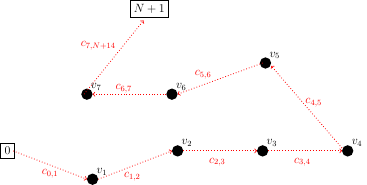
\includegraphics[width=0.8\textwidth]{CSP.png}
% \label{CSP}
% \begin{center}
% Fonte: Elaborada pelo autor
% \end{center}
% \end{figure}

%O objetivo do \ac{CSP} é encontrar todos vértices entre $0$ e $N+1$, tais que todas as tarefas estejam no mesmo caminho, o tempo de trabalho não exceda o tempo total $T$ e o custo total do caminho determinado pelas tarefas executadas seja mínimo. 
% Levando em consideração que cada tarefa pode ser executada apenas uma vez, o custo total associado a cada solução viável é definido pela soma dos custos para realizar cada tarefa $f$, como pode ser visto equação \ref{eqsum}:

% \begin{equation} \label{eqsum}
% 	\sum_{i=1}^{F} c_{f}
%  \end{equation}

% Uma aplicação prática do Crew scheduling problem é o  \textit{Home Care Crew Scheduling Problem}, é um problema no qual uma equipe do \ac{HHCSP} realiza uma série de visitas às casas dos pacientes \cite{rasmussenm:2012}.
%e deve ser encontrado uma solução ótima de forma que todas as visitas sejam feitas no menor tempo possível sem prejudicar a qualidade do atendimento. Este problema foi classificado pelo autor como NP-completo, pois foi verificado a viabilidade em reduzi-lo ao problema do caixeiro viajante, dessa forma, para resolver o problema o autor desenvolveu um algoritmo \textit{branch-and-price}. 

% Uma instância qualquer do problema geral de alocação de equipes pode ser solucionada a partir da variável de decisão $X_{fk}$, tais que, o valor $1$ é associado a uma ligação entre dois vértices, e o valor $0$ determina que não existe uma ligação entre os vértices. Como podemos ver na equação \ref{eqcsp}, que recebe o valor $1$ caso a tarefa $f$ seja associada a equipe $k$ e o valor $0$ caso contrário.

%   \begin{equation} \label{eqcsp}
%   X_{fk} = 
%   \left \{
%   \begin{array}{cc}
%   1, & \mbox{se existe a tarefa $f$ foi alocada a equipe $k$}  \\
%   0, & \mbox{caso contrario} \\
%   \end{array}
%   \right.
%   \end{equation}
  
% A tabela \ref{tarefa_equipe} ilustra um exemplo da solução para o problema de alocação de equipes, no qual cada tarefa $k$ é associada a uma equipe $e_{i}$. 

% \begin{table}[h]
% \centering
% \caption{Tabela: Tarefa X equipes}
% \label{tarefa_equipe}
% \begin{tabular}{l|l|l|l|l}
%    & k1 & k2 & k3 & k4 \\ \hline
% e1 & 0  & 1  & 0  & 0  \\ \hline
% e2 & 0  & 0  & 0  & 1  \\ \hline
% e3 & 0  & 0  & 1  & 0  \\ \hline
% e4 & 1  & 0  & 0  & 0 
% \end{tabular}
% \end{table}

% \subsection{Problema de Alocação de Recursos}

% O problema geral de alocação de recursos consiste em conjunto $R = \{1, 2, ..., r\}$ de recursos que serão escalonados; um custo $c_{r}$ representando o tempo que cada recurso permanecerá alocado, e  um conjunto de processadores  $\Omega = \{1,2, ..., \omega \}$ \cite{ullman:1975}. 
% Como podemos ver na tabela \ref{alocacao_recurso}, no qual o valor é $1$ quando o recurso é alocado no processador $p$ e $0$ quando não é alocado no processador $p$. O objetivo deste problema é executar $k$ recursos dentro do tempo $t$.

% \begin{table}[h]
% \centering
% \caption{Tabela Recurso X Processador \label{alocacao_recurso}}
% \begin{tabular}{l|l|l|l|l}
%    & $\omega1$ & $\omega2$ & $\omega3$ & $\omega4$ \\ \hline
% r1 & 0  & 1  & 0  & 0  \\ \hline
% r2 & 0  & 0  & 0  & 1  \\ \hline
% r3 & 0  & 0  & 1  & 0  \\ \hline
% r4 & 1  & 0  & 0  & 0 
% \end{tabular}
% \end{table}

% O problema de alocação de recursos pode ser solucionado a partir de uma variável de de decisão $X_{r\omega}$, sendo o valor $1$ é atribuído caso o recurso seja associado ao processador, e $0$ se não foi atribuído, como podemos ver na equação \ref{alocacao_recurso}.

%   \begin{equation}
%   \label{alocacao_recurso}
%   X_{rp} = 
%   \left \{
%   \begin{array}{cc}
%   1, & \mbox{ se o recurso $r$ foi alocado ao processador $p$}  \\
%   0, & \mbox{caso contrario} \\
%   \end{array}
%   \right.
%   \end{equation}

\section{Problema do caixeiro viajante}

%O \ac{PCV} é um problema de otimização combinatória no qual, dado um conjunto de cidades e as distâncias entre elas, o objetivo é encontrar o caminho de custo mínimo que passe por cada cidade exatamente uma vez \cite{goyal:2010}.

Seja um grafo $G = (V,A)$, no qual $V$ é um conjunto de vértices e $A$ é um conjunto de arestas, e seja $\tau:V\times V \rightarrow \mathds{R}$ uma função que associa cada par de vértices a uma distância. O \ac{PCV} consiste em determinar um circuito de tamanho mínimo que passa por cada vértice apenas uma vez. Esse circuito é conhecido como um circuito Hamiltoniano \cite{laporte:1992}.

São estudadas diversas variações do \ac{PCV} existindo várias aplicações práticas para o problema, porém neste trabalho serão descritos o \ac{PMCV} e do \ac{PCVJT}. O \ac{PMCV} é uma generalização do \ac{PCV} em que considera um conjunto de caixeiros viajantes, e tem como objetivo determinar, para cada caixeiro, uma rota de custo mínimo onde cada cidade deve ser visitada uma única vez por um único caixeiro viajante~\cite{meng:2012}.  Já no \ac{PCVJT} cada cliente possui um tempo de serviço delimitado por uma janela de tempo definindo o tempo de início e fim do atendimento. As visitas devem ser realizadas respeitando a janela de tempo. O \ac{PCVJT} tem como objetivo encontrar um circuito de custo mínimo, começando e terminando no mesmo depósito e visitando a um conjunto de clientes uma única vez respeitando a janela de tempo de visitação. \cite{urrutia:2010}.

<<<<<<< HEAD
%Seja grafo $G = (V,A,\tau)$, no qual $V = \{v_1, v_2, ..., v_{|V|}\}$ é um conjunto de vértice onde cada um dos seus elementos está associado a uma cidade, e $A = \{ v_i,v_j: v_i,v_j \in V, i \neq j \}$ é uma aresta com uma matriz custo não negativo $C = \{c_{ij}: o \ peso \ de \ (v_i,v_j)\}$. A distância entre $v_i$ e $v_j$ é denotada por $w_{ij}$. 
=======
Seja grafo $G = (V,A,C)$, no qual $V = \{v_1, v_2, ..., v_{|V|}\}$ é um conjunto de vértice onde cada um dos seus elementos está associado a uma cidade, e $A = \{(v_i,v_j): v_i,v_j \in V, i \neq j \}$ é um conjunto de arestas com uma matriz custo não negativo $C = \{c_{ij}: o \ peso \ de \ (v_i,v_j)\}$. A distância entre $v_i$ e $v_j$ é denotada por $c_{ij}$. O \ac{PMCV}, tem como objetivo determinar um conjunto de rotas de custo mínimo que serão percorridas por um conjunto de Caixeiros Viajantes \cite{meng:2012}. 
>>>>>>> bf11a0f8ae334fbc15fd76daf22b0b0f7918b723

%Seja $G=(V,A)$ um grafo, onde $V = \{v_0, v_1, ..., v_{|V|} \}$ é um conjunto de nós, sendo que o nó $0$ representa o depósito e $A = \{ (i,j): i,j \in V, i \neq j \}$ é um conjunto de arestas. O custo de viajar de $i$ para $j$ é representado por $c_{ij}$. Cada cliente $i$ possui uma janela de tempo associada $[e_i, l_i]$, na qual $e_i$ e $l_i$representam o tempo de início e final do atendimento respectivamente. O \ac{PCVJT} consiste em encontrar um circuito hamiltoniano a partir do depósito que satisfaça todas as janelas de tempo e minimize a distância total percorrida\cite{urrutia:2010}.

\section{Problema de roteamento de veículos}

No \ac{PRV} tem como objetivo encontrar uma rota com custo mínimo de modo que seja cumprida a demanda dos clientes. A rota começa e termina no depósito e cada local é visitado apenas uma vez. Cada local é visitado uma vez, e cada veículo possui uma capacidade limitada \cite{gold:2008}.

Seja um conjunto de clientes $Q = \{q_1, q_2, ..., q_{|Q|}\}$, que residem em locais $W = \{w_0, w_1, w_2, ..., w_{|W|}\}$ diferentes. Cada par de locais $(i,j)$, onde  $i,j \in W$ e $i \neq j$, é associado a um tempo de translado $\tau$ e uma distância $u_{ij}$. O depósito, local de onde os veículos partem e retornam, é denotado por $w_0$.
Os clientes são atendidos a partir de um depósito com uma frota  homogênea $Z = \{1, 2, ..., z_{|Z|}\}$ de veículos com capacidade uniforme $y$~\cite{gold:2008}.

O Problema de Roteamento de Veículo com Janela de tempo, o \ac{VRPTW}, assim como o \ac{VRP}, consiste em encontrar um conjunto de rotas com custo mínimo, porém cada cliente $q$ possui uma janela de tempo $[e_{q}, l_{q}]$, sendo $e_{q}$ o tempo de início do atendimento e $l_{q}$ o tempo do fim do atendimento~\cite{gold:2008}.
\xchapter{Problemas de escalonamento e roteamento na área da saúde}
{ }

\presetkeys%
    {todonotes}%
    {inline,backgroundcolor=yellow}{}
 %\todo{}
%\section{Escalonamento e roteamento de equipes de enfermagem}


\section{Problema de Escalonamento de Enfermeiras}

%No restante do texto utilizaremos o termo enfermeiras como uma nomenclatura genérica a todos os profissionais de saúde que possam estar envolvidos no Serviço de Atendimento Domiciliar e termo cliente para todas as pessoas que recebam qualquer atendimento de um profissional do \ac{SAD}.

O \ac{PEE}, conhecido como \ac{NSP}, é um problema de pesquisa operacional que consiste em encontrar uma atribuição de enfermeiras a turnos respeitando a um conjunto de restrições \cite{ioanis:2015}.

Seja $E = \{e_1, e_2, \ldots, e_{|N|}\}$ um conjunto de enfermeiras, Seja $D = \{d_1, d_2, ..., d_{|D|}\}$ um conjunto de dias, seja $F = \{ f_1, f_2, ..., F_{|F|} \}$ um conjunto de tarefas e seja $B$ um conjunto de turnos, onde cada elemento de $B$ está mapeado da seguinte forma: ($M$; matutino), ($V$; vespertino), ($N$; noturno) e ($-$; folga).

Uma solução para o \ac{PEE} pode ser representada por uma matriz $M_{ND}$, na qual cada célula $m_{n_i,d_j}$ contém a atribuição para o turno $t\in B $ que deverá ser comprido pela enfermeira $n$ no dia $d$.


Na Tabela~\ref{enfermeira_dia}, é apresentado um exemplo de escalonamento de enfermeiros cujos valores $n_1$, $n_2$ e $n_3$ representam os enfermeiros escalonados no período de sete dias sendo representados pelos valores $d_1$, $d_2$, $d_3$,$d_4$, $d_5$, $d_6$, $d_7$.

\begin{table}[ht]
 \centering
\caption{Exemplo de escalonamento de três enfermeiras no horizonte de sete dias de trabalho \label{enfermeira_dia}}
\begin{tabular}{r|l|l|l|l|l|l|l}
  	   & $d_1$ & $d_2$ & $d_3$ & $d_4$ & $d_5$ & $d_6$ & $d_7$ \\ \hline
 $n_1$ & $M$  & $V$  & $N$  & $M$  & $V$  & $V$  & $-$ \\ \hline
 $n_2$ & $V$  & $-$  & $M$  & $N$  & $N$  & $-$  & $V$\\ \hline
 $n_3$ & $M$  & $M$  & $V$  & $N$  & $-$  & $M$  & $V$
\end{tabular}
\end{table}


\section{O Problema de Roteamento de Enfermeiras}

Seja um conjunto de enfermeiras $N = \{n_1, n_2, ..., n_{|N|}\}$ , um conjunto de locais $W = \{w_0, w_1, w_2, ..., w_{|W|}\}$, sendo que $w_0$ representa o centro do Serviço de Atenção Domiciliar, seja um conjunto $Q = \{q_1, q_2, ..., q_{|Q|}\}$ de clientes e um conjunto de tarefas $F = \{ f_1, f_2, ..., f_{|F|}\}$.  
Uma solução para o \ac{PEE} pode ser representada por um grafo completo $G = (V, A)$, no qual $V = \{0\} \cup Q$ é um conjunto de vértices sendo que cada vértice representa um cliente $q$ que deve ser visitado pela enfermeira $n$, e $A = \{ (i,j): i \in V, j \in V, i \neq j \}$ é o conjunto de arestas, que representa o translado entre os locais $w_i$ e $w_j$, com tempo de viagem $t_{ij}$ associado ao translado de cada enfermeira do local $w_i$ ao local $w_j$ \cite{mansini:2016}.

O \ac{PEE} consiste em determinar um cronograma que atribui a cada enfermeira $n$ quais clientes $q$ devem ser visitados e qual tarefa $f$ deve ser realizada, respeitando a um conjunto de restrições\cite{mansini:2016}.

\section{Serviço de Atenção domiciliar}

O Serviço de Atenção Domiciliar também conhecido como \ac{HHC} oferece atendimento médico à pacientes em suas residências. 

\subsection{Problema de Escalonamento de Equipe de Serviço de Atenção Domiciliar}

O Escalonamento de Equipe de Serviço de Atenção Domiciliar, conhecido como \ac{HHCSP}, consiste em alocar um conjunto heterogêneo de profissionais de saúde $P = \{ p_1, p_2 ..., p_{|P|} \}$  que realizam visitas a um conjunto de pacientes  $G = \{ g_1, g_2 ..., g_{|G|} \}$, sendo que cada visita realizada a um paciente $g \in G$ por um profissional de saúde $p \in P$ possui a duração de tempo definida como $[e_{g}, l_{g}]$, com $e_{g}$ representando o tempo de chegada e $l_{g}$ representando o tempo de partida do profissional de saúde $p$. A viagem entre as residências de dois pacientes $i$ e $j$  possui o custo $c_{ij}$~\cite{rasmussenm:2012}.   

O \ac{HHCSP} tem como objetivo realizar o escalonamento e roteamento da equipe de atenção domiciliar de forma a gerar resultados eficientes~\cite{bachouch:2010}.


\subsection{Problema de Escalonamento e Roteamento de Equipe de Serviço de Atenção Domiciliar}

O Problema de Escalonamento e Roteamento de Equipe de Serviço de Atenção Domiciliar, também conhecido como \ac{HHCRSP} consiste em  encontrar um cronograma, de modo que cada profissional de saúde visite um conjunto de pacientes , faça uma pausa para almoço e finalize o expediente, tudo dentro da janela de tempo do profissional de saúde. O objetivo do \ac{HHCRSP} é maximizar a quantidade de trabalho minimizando a quantidade de viagem necessária. \cite{cheng:98}

Uma solução para o \ac{HHCRSP} pode ser representada em um grafo, simples e direcionado $G = (V,A)$. O conjunto de nós $V$, consiste em três conjuntos disjuntos: Um conjunto $P = \{ p_1, p_2 ..., p_{|P|} \}$ de profissionais de saúde, um conjunto $Q = \{ q_1, q_2 ..., q_{|Q|} \}$ de clientes e um conjunto L de pausas. O conjunto de arcos A, é baseado em uma noção de compatibilidade. Existe uma relação binária entre cada profissional de saúde e qualquer outro nó. Em outras palavras, a cada enfermeiro é permitido ou impedido de visitar um nó em V. Sendo que o gráfico não contém loops nem arcos entre dois nós de enfermeiro ou entre dois nós de almoço.\cite{cheng:98}. 

Cada profissional de saúde $p \in P$ possui uma janela de tempo $[e_p, l_p]$ que indica o horário de início e fim do seu turno. Cada cliente $q \in Q$ possui o tempo $d_q$, que indica o tempo necessário para fornecer cuidados de saúde ao cliente, e uma janela de tempo $[e_q,l_q]$ no qual $e_q$ é o limite inferior para o tempo de início do atendimento ao cliente $q$ e  $l_q$ é o limite superior do início do atendimento ao paciente $q$. O conjunto de pausas consiste em um nó único para cada profissional de saúde onde cada pausa possui uma duração e uma janela de tempo \cite{cheng:98}.
\xchapter{Revisão sistemática de literatura}
{ }%Revisão sistemática de literatura}

\section{Protocolo da revisão sistemática de literatura}

A revisão sistemática de literatura é um método de seleção de artigos a partir de um protocolo de busca que tem como objetivos resumir evidências empíricas, identificar lacunas existentes nas pesquisas realizadas até o momento e fornecer estruturas para realizar novas pesquisas. Uma revisão sistemática de literatura é composta por três fases: planejamento da revisão, condução da revisão e análise dos resultados~ \cite{Kitchenham:2007} .

Na fase do planejamento é escolhido qual tema será estudado. define-se a pergunta de pesquisa, que deverá ser respondida após a análise dos artigos estudados. Seleciona-se as palavras chaves para a criação da string de busca que será utilizada nas bases de dados escolhidas pelo pesquisador e por fim devem ser escolhidos os critérios de inclusão e de exclusão.

Na fase de condução da revisão, as strings de busca criadas deverão ser aplicadas nas bases de dados escolhidas na fase anterior.
Após adquirir o material através da aplicação das strings de busca, os resultados retornados são classificados em dois grupos: os artigos que foram aceitos e os que foram rejeitados.

A classificação é realizada através da aplicação dos critérios de inclusão e de exclusão escolhidos na fase anterior.
Quanto à escolha dos critérios de inclusão e de exclusão que serão aplicados no artigo, cabe enfatizar que deve-se seguir a  seguinte regra: Se um artigo se encaixar em pelo menos um critério de exclusão, este deverá ser eliminado do grupo de artigos aceitos, mesmo que se encaixe em algum critério de inclusão, e para um artigo pertencer ao conjunto de artigos aceitos devem satisfazer a todos os critério de inclusão e a nenhum critério de exclusão~\cite{Kitchenham:2007}. 

Essa revisão sistemática de literatura tem como propósito: identificar as lacunas existentes no Problema de Roteamento e Escalonamento da Equipe de Atenção Domiciliar e auxiliar na construção de novas soluções para o problema. 

Além dos artigos coletados a partir da chave de busca, outros materiais também foram utilizados para complementar a pesquisa, tais como artigos encontrados a partir de outras bases de dados ou a partir de outras strings de busca, literatura cinza ou livros.

\section{Execução do Mapeamento Sistemático}

O objetivo desse mapeamento sistemático é buscar materiais para investigar a possibilidade propor uma solução heurística para o Problema de Escalonamento e Roteamento de Profissionais de Saúde, de forma que seja possível aumentar  o número de clientes atendidos e reduzir o tempo de transporte da equipe de profissionais de saúde. 
A partir do objetivo da pesquisa foi encontrado a seguinte questão de pesquisa:~\emph{É possível maximizar o número de visitas da equipe de atendimento domiciliar a partir da aplicação de soluções heurísticas?}

Para responder a questão de pesquisa foram examinados trabalhos sobre utilização de heurísticas e meta-heurísticas aplicadas ao escalonamento e roteamento  de equipes de enfermeiras e de atendimento domiciliar, tendo como grupo de controle heurísticas relacionadas com o problema.

O resultados esperados ao final da pesquisa é: A identificação de lacunas existentes no Problema de Escalonamento e Roteamento da Equipe de Atenção Domiciliar e facilitar o acesso das heurísticas já elaboradas por outros pesquisadores para que dessa maneira facilite a construção de novas soluções para o problema.

Para a elaboração da pesquisa foram utilizadas as seguintes palavras chave: \textit{``home health care''}, \textit{``home care'', ``nurse scheduling''} e \textit{``nurse routing''}, organizadas na seguinte string de busca: \textit{``(``home health care'' OR ``home care'') AND (``routing OR scheduling'')''} e \textit{``nurse AND (routing OR scheduling)''}. 

A Pesquisa foi restrita a artigos escritos na língua inglesa e portuguesa, selecionados a partir seguintes bases de pesquisa: \textit{Science Direct, Springer}, \textit{IEEE Xplore}, \textit{Scopus} e \textit{ACM Digital Library}. Além dos artigos selecionados a partir da strings de busca nas bases citadas, a pesquisa conta com outros materiais, tais como livros, materiais retirados da literatura cinza e artigos adquiridos de forma ad-oc.

A pesquisa realizada a partir da string de busca retornou 151 resultados distribuídos da seguinte forma: 73 artigos da \textit{Science Direct}, 50 artigos do \textit{IEEE Xplore}, 16 artigos da \textit{Springer}, 7 artigos da \textit{Scopus} e 5 artigos da \textit{ACM digital Library}.% como pode ser observado na Figura~\ref{base_de_dados_de_origem}.

%Colocar figura nos slides
% \begin{figure}[H]
% \begin{center}
% 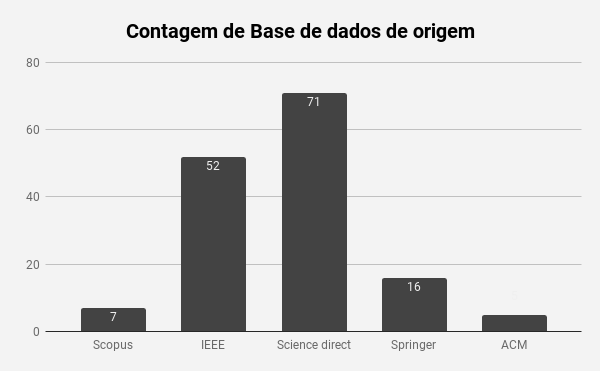
\includegraphics[width=0.6 \textwidth]{contagem_base_de_dados_de_origem.png}
% \caption{Contagem de artigos por bases de dados \label{base_de_dados_de_origem}}
% \end{center}
% \end{figure}

Após a realização da busca dos artigos nas bases de dados especificadas, os artigos encontrados foram selecionados segundo os seguintes critérios de inclusão e de exclusão.

\textbf{Critérios de inclusão:}
\begin{itemize}
\item Artigos que possuam foco em problemas de escalonamento de profissionais de saúde;
\item Artigos que possuam foco em problemas roteamento de veículos das equipes de profissionais de saúde;
\item Artigos publicados em revistas ou conferências.
\item Artigos da área de Pesquisa Operacional
\end{itemize}

\textbf{Critérios de exclusão:}
\begin{itemize}
\item Artigos que não estejam em inglês ou português;
\item Artigos inacessíveis ou indisponíveis;
\item Artigos duplicados;
\item Artigos que não sejam da área de áreas médicas;
\item Artigos que não possuam heurísticas para o \ac{HHCP} e suas variações;
\item Revisões de literatura.
\end{itemize}

Após a aplicação dos critérios de inclusão e de exclusão nos 151 artigos coletados, 41 artigos foram aceitos por atenderem a todos os critérios de inclusão e 110 artigos foram rejeitados por se encaixarem em pelo menos um critério de exclusão. %Como pode ser observado na figura \ref{status}

%colocar figura nos slides
% \begin{figure}[H]
% \begin{center}
% 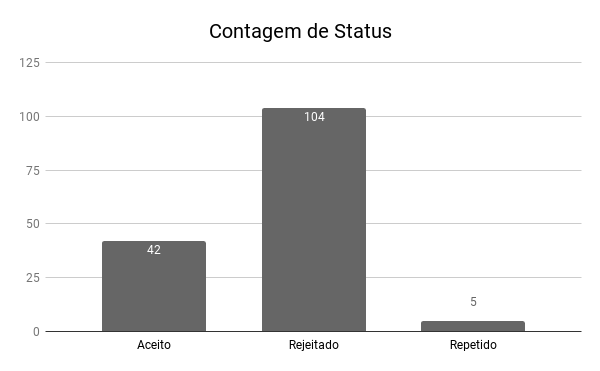
\includegraphics[width=0.8 \textwidth]{status.png}
% \caption{Contagem bases de dados \label{status}}
% \end{center}
% \end{figure}

\section{Resumo dos resultados encontrados}


\cite{nguyen:2016} apresenta uma solução meta-heurística com base em Algoritmos Genéticos para solucionar o \ac{HHCP}. Em sua abordagem são utilizadas duas substituições: A primeira substitui as soluções anteriores aleatoriamente e a segunda substitui as piores soluções. Os testes computacionais foram realizados com instâncias baseadas em dados históricos reais de uma empresa de \textit{Home Care} que opera na Suíça.

% Foi proposta uma solução para o \ac{NSP}, baseado em Algoritmos Genéticos Cooperativos por \cite{ohki:2008}, tendo como solução um horário de enfermagem eficiente. Alguns anos depois \cite{ohki:2011} aplicou uma técnica de Penalização Ponderada em Algoritmos Genéticos Cooperativos para solucionar o \ac{NSP}, tendo como resultado o agendamento de horário realizado em um décimo do tempo, quando comparado com técnicas convencionais.

% Foi apresentado uma abordagem baseada em Memória Externa, junto com Algoritmos Genéticos Multi-Objetivos para resolver o \ac{NSP} por\cite{ahmet:2009}, tendo como resultado melhores soluções quando comparadas com os Algoritmos Genéticos Multi-Objetivos sem memória. 

Foi desenvolvido uma modelagem matemática em dois estágios para o \ac{NSP} por \cite{tsai:2009}, sendo que na primeira etapa organiza-se o horário de trabalho e de folga de enfermeiros, e o Algoritmo Genético é usado para resolver os horários. No segundo estágio o cronograma dos enfermeiros foi organizado e o Algoritmo Genético foi utilizado para resolver o horário ideal. O autor realizou um estudo de caso empírico, tendo como resultados que o Algoritmo Genético pode ser uma ferramenta eficiente para resolver o \ac{NSP}.

Foi elaborada uma heurística para o \textit{Home Care Crew Scheduling Problem} baseada em Algoritmo Evolutivo utilizando quatro instâncias diferentes do mundo real fornecidas por uma empresa privada. Os resultados mostram, por um lado, que as soluções da empresa estão claramente superadas pela nossa proposta algorítmica e, por outro lado, que a paralelização proposta permite ao algoritmo abordar adequadamente instâncias com mais de 10000 serviços \cite{luna:2013}. 

% Baseado na teoria Fuzzy, \cite{mutingi:2013}  elaborou uma heurística para o escalonamento de equipe de atendimento domiciliar, utilizando o método de Enxame de Particulas Fuzzy.
Em busca de encontrar a solução para o \ac{HHCSP}, \cite{trautsamwieser:2014} elaborou uma heurística baseada no método \textit{Branch-Price-and-Cut}, em testes computacionais o autor testou sua abordagem com instâncias baseadas em mais de nove enfermeiras, 45 clientes e 203 visitas durante a semana.

Uma abordagem baseada em Programação por Restrição Lógica para o \ac{HHCP} foi elaborada por \cite{cattafi:2012}, baseado na realidade enfrentada pela cidade de Ferrara na Itália, onde o problema é resolvido manualmente. O autor formalizou o problema através da interação com a equipe de enfermagem do hospital da cidade, tendo como objetivo reduzir as disparidades na jornada de trabalho das enfermeiras.

Foi descrito um método de agendar tarefas e equilibrar a carga de trabalho dos profissionais do \ac{HHCSP} baseado na realidade dos hospitais da França por \cite{bachouch:2010}. 
Foi desenvolvido uma solução heurística para solucionar o \textit{Crew Constrained Home Care Routing Problem with Time Windows} por \cite{tozlu:2016}, descrevendo o problema a partir de um 0-1 \textit{mixed Integer Programming} e em seguida foi gerado aleatoriamente um conjunto de instâncias e resolvidos a partir do \textit{Variable Neighbourhood Search}. 

Para encontrar uma boa solução para o \ac{NSP} \cite{kundu:2008} converteu o problema no Problema de Satisfação de Restrição e aplicou a técnica de Busca Local Gulosa incorporada com a Lista Tabu, testando também outras soluções baseadas no Restrição e aplicou o \textit{Simulated Anealing}, Algoritmo Genético, obtendo melhores resultados a partir da Busca Local Gulosa.
Foi proposto por \cite{trabelsi:2012} um modelos de escalonamento baseado em Programação Interira Linear para fornecer soluções para o planejamento de curto prazo para o \ac{HHC}.

Foi encontrada uma solução para o \textit{Therapist Routing and Scheduling Problem} a partir de um algoritmo sequencial adaptativo de Busca Gulosa Randomizada, o GRASP por \cite{bard:2012}, para testar sua solução foram realizados testes com dados reais fornecidos por uma empresa de reabilitação dos EUA, obtendo como resultado reduções de custo com uma média de cerca de 18,09\%.

Foi elaborado por \cite{Decerle:2016} uma heurística de duas fases para o \ac{HHCRSP} com o objetivo de reduzir custos relacionados a transporte e a horas trabalhadas pelos profissionais de saúde. Para solucionar o problema foram sugeridos duas abordagens: Um método de solução monofásica onde o conjunto de dados completo é considerado como entrada para encontrar a melhor solução para o problema e uma meta-heurística em duas fases para distinguir o agendamento das enfermeiras e os funcionários assistivos sem licença. As abordagens são então experimentadas em várias instâncias de diferentes tamanhos, obtidas a partir de dois escritórios de \textit{Home Care} para compará-las.

A solução heurística apresentada para o \ac{HHCP} por \cite{Bertels:2006} é baseada na combinação de Programação Linear, Programação por Restrição e meta-heurísticas. As instâncias utilizadas para gerar a solução foram obtidas a partir de 10 cenários sintéticos, contendo entre 20 e 50 profissionais e entre 111 e 326 trabalhos.

Foi elaborado por \cite{gambini:2012} uma solução heurística baseada em Programação Inteira para o \textit{International Nurse Rostering Competition}.
Foi elaborada uma proposta de solução heurística baseada em Programação por Restrição Ponderada para o Second \textit{International Nurse Rostering Competition} por \cite{santos:2015}.

% Foi elaborada uma heurística baseada em Busca Local para o \ac{NSP}, por \cite{inafune:2016}, os autores utilizaram em seus experimentos instancias reais, colhidas de um hospital.
% Foi elaborado por \cite{mutingi:2015} uma abordagem baseada em Algoritmo de Metamorfose Fuzzy para o \ac{NSP}, utilizando dados do mundo real e encontrados na literatura estudada.

Uma abordagem heurística para o \ac{NSP}, baseada em Satisfação de Preferência Balanceada foi elaborada por \cite{constantino:2011}. O algoritmo elaborado possui duas fases: Na primeira fase é construída a solução inicial, resolvendo o problema sucessivo de atribuição por estrangulamento e na segunda fase são aplicados dois procedimentos de melhoria baseados em etapas de reatribuição. Os testes computacionais foram realizados com instâncias do \textit{Standard Benchmark Bataset} e a partir dos experimentos os autores concluíram que o método utilizado gerou resultados efetivos e eficientes para solucionar o problema.

% Foi formulada uma nova solução para o \ac{NSP} por \cite{baskaran:2014} utilizando o \textit{Branch and Bound} e o solucionador de simplex duplo, obtendo bons resultados a partir da aplicação de instâncias do mundo real.
% Uma abordagem colaborativa para resolver o \ac{NSP} foi elaborada por \cite{cares:2013} usando uma formulação de programação não-linear. Neste modelo, a função a ser otimizada é não-linear, esta função é focada em procurar uma solução que minimiza as diferenças entre os enfermeiros. Os autores utilizaram instâncias do mundo real para realizar os testes, obtendo resultados efetivos.

O algoritmo de Busca Harmônica  tem sido utilizado para solucionar problemas de otimização, este método funciona a partir da imitação do processo de improvisação musical. Foi elaborada uma abordagem meta-heurística baseada em Busca Harmônica para o \ac{NSP}, por\cite{awadallah:2011}. Para realizar os testes computacionais foram utilizados dados do \textit{ International Nurse Rostering Competition 2010}, retornando bons resultados.

Foi desenvolvida um abordagem baseada em Programação Inteira Binária para gerar uma solução heurística para o \ac{NSP}, por \cite{Zen-El-Din:2012}. O autor realizou um estudo de caso  na unidade de terapia intensiva no Hospital do Cairo, sendo que os dados foram coletados de enfermeiros-chefe, supervisores, enfermeiros e assistentes.

Uma abordagem para resolver o \ac{NSP} em um hospital público na França foi desenvolvida por \cite{altamirano:2010} baseada em otimização por Enxame de Partículas, tendo resultados semelhantes em tempo computacional ao método de Programação Inteira e Programação por Restrição.

Foi elaborada uma heurística para o \ac{NSP} baseada em Vetorização de Matrizes por \cite{yindong:2008}, após experimentos computacionais foram obtidas boas soluções para 10 instâncias de dados reais de programação de enfermagem. 
Foi elaborado um modelo baseado em Lógica Fuzzy para solucionar o \ac{NSP} por \cite{topaloglu:2010}.
Um modelo de Programação Inteira Multi Objetivo para o \ac{NSP} foi proposto por \cite{cetin:2015}, em seguida os autores elaboram uma abordagem baseada em Lógica Fuzzy e aplicam a um estudo de cado em um hospital em Konya, na Turquia.

Foi elaborado por \cite{gutjahra:2007} uma heurística baseada em Colônia de Formiga para resolver o \ac{NSP} no \textit{Vienna Hospital Compound} na Áustria. Após realizar experimentos, foi observado que o algoritmo proposto alcança melhorias significativas em comparação a um algoritmo de abordagem gulosa.
Uma abordagem de otimização de Enxame de Particulas é proposto por \cite{wu:2015} para encontrar uma boa solução para o \ac{NRP}, tendo como estudo de caso um hospital de Taiwan. 

% É apresentado um modelo que integra  agendamento da enfermeira e do quarto cirúrgico e em seguida é mostrado por \cite{belien:2008} uma a abordagem da técnica de geração de coluna, um dos métodos exatos mais empregados para resolver problemas de programação de enfermeiros, pode fazer face facilmente a essa extensão de modelo.

Foi apresentado por \cite{lu:2012} um método baseado em \textit{Adaptive Neighborhood Search} para resolver o \ac{NSP} para do \textit{ First International Nurse Rostering Competition}.  Os resultados computacionais avaliados nos três conjuntos de 60 instâncias da competição mostram que o algoritmo utilizado melhora os resultados mais conhecidos por 12 instâncias ao combinar os melhores limites para outras 39 instâncias.

% Foi elaborado por \cite{burke:2010} um modelo de Programação Inteira e \textit{Variable Neighbourhood Search} para o Problema de Seleção de Enfermeiras, tendo como resultado boas soluções quando comparado com as soluções elaboradas com Algoritmos Genéticos e Busca em Vizinhança.

% Foi elaborado para a  Primeira Competição Internacional de Enfermagem (INRC2010),  uma abordagem em duas fases por \cite{valouxis:2012}, em sua solução na primeira fase, a carga de trabalho para cada enfermeiro e para cada dia da semana foi decidida, enquanto na segunda fase as deslocações diárias específicas foram atribuídas.

%\section{Análise descritiva dos resultados encontrados}

%Na seção anterior foi realizada uma revisão das soluções heurísticas encontradas a apartir da revisão sistemática de literatura, nessa parte serão descritas com mais detalhes algumas soluções heurísticas mais utilizadas pelos autores.

% \subsection{Técnicas de inteligência artificial}

% Vários autores utilizaram técnicas de inteligência artificial para elaborar heurísticas para o \ac{HHCSP} e o \ac{HHCRSP}, podendo citar as técnicas seguintes como as mais utilizadas.

%\subsection{Lógica Fuzzy}

% \
% \linebreak[4]

%A teoria de conjuntos difusos, do inglês \textit{fuzzy}, trabalha com modelos de conjunto cujo seus elementos possuem um determinado grau de pertinência a este conjunto, não aceitando valores booleanos, como acontece em conjuntos precisos, ou seja, que não são difusos \cite{mutingi:2013}.

%Para melhor entendimento sobre a teoria de conjuntos difusos, \citeonline{mutingi:2013} descreve a seguinte diferença entre os conjuntos:

%Seja um conjunto universo $X$ composto por elementos $x$, e o subconjunto $A$ do conjunto universo $X$, tal que $A \subseteq X$. 

%O elemento $x$ é um membro de um conjunto preciso se é definido pela função transformação $\mu_{A}$ a partir de $X$ em {0,1}, desde que:

% \begin{equation}
%  \mu_{A}(x) = 
%  \left \{
%  \begin{array}{cc}
%  1, & se \ x \ \in \ A  \\
%  0, & se \ x \ \notin \ A \\
%  \end{array}
%  \right.
%  \end{equation} 

%Em um conjunto difuso, o elemento $x \in A$  é definido por $\mu_{A}(x) \in [0,1]$, cujo cada elemento em X possui o valor dentro do intervalo [0,1] sendo que quanto mais próximo o valor de $\mu_{A}(x)$ está de $1$, maior é o grau de pertinência do elemento $x$ em A, e quanto mais próximo de $0$, menor o seu grau de pertinência.


%\subsection{Algoritmos Genéticos \hfill}
% \
% \linebreak[4]

%Algoritmos genéticos pertencem a uma subclasse de algoritmos evolutivos e possuem seu funcionamento baseado na teoria evolutiva da biologia proposta por Darwin. Nas ultimas décadas os algoritmos evolutivos tem sido bastante utilizados para resolver problemas de otimização.~\cite{malhotra:2011} 

%Os algoritmos genéticos contém um cromossomo, um gene, conjunto populacional, um \textit{fitness} e função \textit{fitness}, reprodução, mutação e seleção.

%O funcionamento dos algoritmos genéticos começam com um conjunto solução representado por um conjunto de cromossomos, chamado população, na qual cada cromossomo representa um individuo. As soluções são selecionadas de acordo com sua aptidão para gerar novas soluções, chamadas descendência, cada solução gerada para uma população é utilizada para uma nova população, possivelmente melhor do que a população anterior. 

%O processo utilizado para gerar uma população é repetido até que as condições pré definidas sejam satisfeitas, como pode ser visto no algoritmo~\ref{genetico}.

%\begin{algorithm}[ht]
% \Entrada{$P$} //população inicial \\
% \Saida{individuo que satisfaz a condição pré definida}
%   \Inicio{
%	Selecione uma subpopulacao $P'$
%     \While { $X$ não é satisfeito }{
%        escolha $S_{i}, S_{j} \in P'$ \\
%        $S_{k} \longleftarrow CRUZAMENTO(S_{i}, S_{j})$ \\
%      \eIf{$f(S_{i} \geq f(A_{j})$}{
%        	$S_{melhor} \longleftarrow S_{i}$\\
%        	}{$S_{melhor} \longleftarrow S_{j}$\\} 
%       \eIf{$f(S_{melhor}) \geq f(S_{k})$}{
%       	  $SUBSITUI(S_{melhor}, P)$\\
%        }{não substitui}  
%        $S_{k} \longleftarrow MUTACAO(S_{k})$ \\
%        }
%      \Retorna{$S_{k}$} \\
%   }
% \caption{Algoritmo genético \label{genetico}}
%\end{algorithm}

%O pseudocódigo acima ilustra o funcionamento do Algoritmo Genético, no qual a entrada é uma população P e a saída é um indivíduo $S$. Primeiramente é selecionada uma população inicial $P$ que irá gerar uma nova população. Até que o critério de parada seja satisfeitos, é gerada uma nova população $P'$, subconjunto da população $P$, da seguinte forma: São escolhidos aleatoriamente dois cromossomos $S_{i}$ e $S_{j}$ em cada subpopulação $P'$, estes cromossomos são recombinados a partir do cruzamento dos mesmos, levando a formação de um novo cromossomo $S_{k}$. O cromossomo $S$, representa o valor da função objetivo, dessa forma, quanto menor o valor, melhor será a adequação do indivíduo representado pelo cromossomo. Após a comparação do cromossomo filho com os cromossomos pais, é realizado o procedimento de mutação, gerando uma nova descendência.

%A cada iteração do algoritmo é testado se o indivíduo gerado satisfaz a condição $X$ pré definida, caso as condições sejam satisfeitas, o algoritmo para e retorna o indivíduo, caso contrário ele segue até que alcance alguma outra condição de parada $X$.

%\subsection{Memetic Algorithm}
% \
% \linebreak[4]

%\textit{Memétic Algorithm} são metaheurísticas baseadas em população, compostas por uma estrutura evolutiva e um conjunto de algoritmos de busca local. 
%Apesar de ser utilizado para resolver problemas de otimização, apesar de sua utilização o \textit{Memétic Algorithm} não é proposto como um algoritmo de otimização, mas como uma ampla classe de algoritmos inspirados pela difusão das ideias ideias e compostas por múltiplos operadores existentes~\cite{neri:2012}.  
 
%O \textit{Memétic Algorithm} visa a convergência de uma população para uma solução ótima, como segue:
%Primeiro é realizada a seleção aleatória das soluções candidatas iniciais, chamada de pais, que serão utilizadas para a criação de uma nova solução. Essa seleção é realizada levando em consideração o desempenho das soluções candidatas, quanto melhor o desempenho, maiores são as chances de seleção das soluções.
%A segunda etapa do algoritmo consiste em combinar os pais e criar uma nova solução candidata, mais próxima do resultado esperado.
%Após a geração da nova população, ocorre a fase de mutação, na qual é realizada uma melhoria no novo resultado gerado.   
%A ultima etapa decide se a nova população gerada deve se tornar membro da população e qual solução existente deve ser substituída.

%\subsection{Colônia de formiga}
% \
% \linebreak[4]

%O algoritmo de Colônia de Formigas, possui seu funcionamento baseado no comportamento das formigas na natureza, particularmente no processo realizado por estas ao procurar comida. Quando as formigas vão em busca de comida, elas partem aleatoriamente até encontrar a comida, ao encontrar a comida a formiga retorna para o seu ninho deixando uma trilha de ferormônios, que será seguida pelas outras formigas~\cite{blum:2005}.

%O algoritmo de Colônia de Formigas é descrito como um grafo G = (V,E), onde V consiste em dois nós nomeados $v_{s}$, representando o formigueiro e $v_{d}$, representando a comida; e $E$ representa duas ligações, $e_{1}$ e $e_{2}$ o caminho entre o formigueiro, representado por $v_{s}$ e a comida, representada por $v_{d}$. Sendo que $e_{1}$ representa o caminho mais curto e $e_{2}$ representa o caminho longo. 

%A representação da trilha de ferormônio é modelada da seguinte forma: É introduzido um ferormônio artificial $t_{i}$ para cada duas ligações $e_{i}$, sendo i=1,2; indicando a força da trilha deixada. Por fim, são introduzida formigas artificiais, representadas por $n_{a}$. Para criar o caminho de cada formiga do formigueiro até a comida, ou seja de $v_{s}$ para $v_{d}$, cada formiga que parte do ponto $v_{s}$ é escolhida com probabilidade: 

%\begin{equation}
%P{i} = {t_{i}\over\displaystyle {t_{1}+t_{2} } }, \ para\ i = 1,2
%\end{equation}

%entre os caminhos $e_{1}$ e $e_{2}$ para alcançar a comida $v_{d}$. Se $t_{1} > t_{2}$, a probabilidade do caminho 1 ser escolhido é maior.
%Para criar o caminho de volta para o formigueiro, ou seja, o caminho de $v_{d}$ para $v_{s}$ é utilizado o mesmo caminho criado de $v_{s}$ para $v_{d}$~\cite{blum:2005}.

%\subsection{Algoritmo Guloso}

%Algoritmos Gulosos sempre escolhem a melhor solução para o momento partindo do ótimo local em busca do ótimo global. Apesar deste algoritmo encontrar a solução ótima para vários problemas, nem sempre é possível alcançar a solução ótima a partir da execução deste algoritmo~\cite{Cormen:2009}. 

%Em um Algoritmo Guloso, a cada iteração, um novo elemento do conjunto solução é incorporado a construção da solução parcial até que a solução completa seja obtida. A seleção do próximo elemento que será incorporado é determinado a partir da função gulosa de avaliação. esta função gulosa representa o aumento incremental na função custo para a incorporação deste elemento na solução parcial em construção~\cite{resende:2014}. O critério para estabelecer qual elemento será selecionado é o do elemento menos custoso, como podemos ver no algoritmo~\ref{guloso}.

%\begin{algorithm}[ht]
% \Entrada{$C \neq \emptyset$} //conjunto de candidatos \\
% \Saida{melhor solução segundo o critério guloso}
%   \Inicio{
%   		$S \longleftarrow \emptyset $ //o conjunto solução $S$ está vazio inicialmente \\
%        $C \longleftarrow E $ //inicializa o conjunto $C$ com o conjunto inicial $E$ \\
%     \While {$C \neq \emptyset \wedge \neg solucao(S)$ }{
%        $ x \longleftarrow seleciona(C)$ //seleciona o proximo candidato \\
%        $C \longleftarrow C - x$ //remove x do conjunto de candidatos \\
%        \eIf{Viavel($S + x$)}{
%        	$S \longleftarrow S + x$  //adiciona o candidato ao conjunto solucao\\
%        }{$S \longleftarrow S$} //nao atualiza o conjunto solucao \\
     %}
%     \Retorna{S} //melhor solução segundo o critério guloso \\
%   }
% \caption{Algoritmo guloso  \label{guloso}}
%\end{algorithm}


%\subsection{Greedy Randomized Adaptative Search Procedure}
% \
% \linebreak[4]

%Para descrever o \ac{GRASP} será levado em consideração o problema de otimização combinatorial para minimizar a função $f(s)$ para cada solução $S \in X$, sendo definido a partir de um conjunto inicial finito $E = \{ e_{1}, e_{2}, ..., e_{n} \}$ para um conjunto viável de um conjunto soluções viáveis $X \subseteq 2^E$ e pela função objetiva $f:2^E\rightarrow$. 
%O conjunto de soluções viáveis para o problema é definido a partir do E, a função objetivo e das restrições. 
%O \ac{GRASP} é chamado de adaptativo porque os benefícios associados com cada elemento é atualizado a cada iteração da fase construtiva para refletir as mudanças trazidas pela seleção do elemento anterior.~\citeonline{resende:2014}.

%O \ac{GRASP} é definido por como uma heurística gulosa adaptativa de randomização iterativa constituída por duas fases: Uma fase construtiva e outra fase de busca local~\cite{feo:1995} e~\cite{resende:2014}. 
%Na fase de construção é elaborada uma solução, se esta solução não for viável, poderá ser descartada ou é aplicada uma heurística reparatória para alcançar a viabilidade. Uma vez que a solução viável é obtida, a vizinhança que possui esta solução é investigada até que seja encontrado o mínimo local através da etapa de busca local~\cite{resende:2014}.

% Para descrever o \ac{GRASP} \citeonline{resende:2014} leva em consideração o problema de otimização combinatorial para minimizar a função $f(s)$ para cada solução $S \in X$, sendo definido a partir de um conjunto solução finito $E = \{ e1, e2, ..., en \}$ para um conjunto viável de um conjunto soluções viáveis $X \subseteq 2^E$ e pela função objetiva $f:2^E\rightarrowR$. 
% O conjunto de soluções viáveis para o problema é definido a partir do E, a função objetivo e das restrições~\cite{feo:1995}.

%Para a elaboração da etapa construtiva, na qual solução viável é construída iterativamente, um elemento por vez e a cada iteração a escolha do próximo elemento que será adicionado é determinado pela ordem de todos os elementos candidatos em uma lista que respeita a função gulosa, são utilizados algoritmos randomizados.
%Os algoritmos randomizados são importantes para gerar o espaço de busca inicial em uma vizinhança, quebrar loops, habilitar trajetórias diferentes para seguir em uma mesma solução inicial ou simplificar diferentes partes em uma vizinhança extensa~\cite{resende:2014}. 

%Na fase de busca local, é utilizado um algoritmo de busca local que funciona de maneira iterativa, substituindo sucessivamente a solução corrente pela melhor solução encontrada na vizinhança, determinando quando a melhor solução não é encontrada na vizinhança.

%O algoritmo~\ref{grasp} ilustra o funcionamento do \ac{GRASP}, no qual recebe um conjunto de valores candidatos, o máximo de iterações e é utilizado um valor inicial pseudo-aleatório chamado semente e retorna a melhor solução encontrada.

%\begin{algorithm}[h]
% \Entrada{$C, m, s$} //conjunto de candidatos C, maximo de iteracoes m, e semente s \\
% \Saida{melhor solução}
%   \Inicio{
%		\For{$k \longleftarrow 1$ \KwTo $m$ }{
%        	$solucao \longleftarrow  %solucaoConstrutiva(C, s)$ \\
%            $solucao \longleftarrow  %buscaLocal(solucao, melhorSolucao)$\\
%        }
	
%     \Retorna{melhorSolucao} //melhor solução %segundo o critério guloso \\
%   }
% \caption{GRASP \label{grasp}}
%\end{algorithm}

%No contexto de atendimento do \ac{HHCSP} a heurística gulosa foi utilizada por alguns pesquisadores como~\cite{yuan:2015} e~\cite{bard:2012}, que utilizou o \ac{GRASP} para solucionar o \textit{Therapist Routing and Scheduling Problem}, problema semelhante ao \ac{HHCRSP}.

%\subsection{Adaptative Iterated Construction Search}
%não tem artigos falando sobre

%O \ac{AICS}, assim como o~\ac{GRASP}, é um algoritmo utilizado para resolver problemas de otimização, pertencente à sub-área de otimização cujo o conjunto de soluções viáveis é ou pode ser reduzido a um conjunto discreto. 
%Esse algoritmo utiliza a experiência adquirida em soluções passadas para gerar soluções melhores. 
%Uma forma de implementar esta ideia é associar pesos com possíveis decisões que serão tomadas durante o processo construtivo. Estes pesos são adaptados através de múltiplas iterações do processo de busca para refletir a experiência de iterações passadas~\cite{hoss:2005}.

%O funcionamento do \ac{AICS} é dividido em três fases: Construtiva, busca local e adaptação dos pesos. 
%Na fase construtiva, um processo de busca é utilizado para gerar uma solução candidata $s$, em seguida. 
%Na fase de busca local é realizada uma perturbação em $s$, produzindo a solução ótima local $s'$. 
%Por fim, os pesos são adaptados baseados nos componentes da solução utilizados em $s'$ e na qualidade da solução $s'$.
%O processo de busca construtiva utiliza o peso $w$ e alguma função heurística $h$ sobre os componentes da solução selecionados de componentes probabilisticamente selecionados para ampliar a solução parcial candidata atual. 
%Na fase de ajuste de pesos, é realizado um aumento dos pesos que correspondem aos componentes da solução em $s'$, podendo ser utilizados do histórico de busca~\cite{hoss:2005}.

%\subsection{Dynamic Local Search}

%A ideia geral do \ac{DLS} é buscar através do espaço de soluções viáveis e melhorar o retorno da função objetivo, realizando movimentos de subida para escapar de mínimos locais. Uma vantagem deste método é a rápia convergência em direção ao ótimo global da função objetivo sem utilizar derivadas de gradiente ou de ordem superior~\cite{amin:1997}.

%A ideia básica do algoritmo é explorar através do espaço local e global simultaneamente, permitindo a exploração detalhada de áreas de ótimos locais escapando destas.

%\subsection{Busca Tabu}
	
%A Busca Tabu é uma meta-heurística utilizada para guiar uma busca local na exploração do espaço solução além do ótimo local, sendo considerado um método cujo principal objetivo é minimizar a função objetivo $f(x)$~\cite{marti:2013}. A busca tabu é importante para resolver problemas de otimização utilizando uma estrutura de memória flexível~\cite{glover:1990}.
  
%Na busca tabu, é realizada uma busca na estrutura de vizinhança $N$, na qual a solução $x \in N(x)$ encontrada é trocada por uma solução melhor $x' \in N(x)$ atingida a partir de uma operação chamada movimento. 
%Este método permite apenas movimentos que melhorem o valor da função objetivo atual e a execução do algoritmo termina quando não são mais encontradas soluções melhores~\cite{marti:2013}. 
% O autor afirma que Uma falha existente no método decrescente é que o ótimo local, na maioria dos casos, não será o ótimo global, ou seja, geralmente não irá minimizar $f(x)$ em todas as soluções $x$ pertencentes a $X$.

%Na Busca Tabu são utilizados atributos flexíveis baseados em estruturas de memória que permitem a exploração do critério de avaliação e de informações de busca armazenadas; um mecanismo de controle associado, para empregar a estrutura de memória, com base na interação entre condições que restringem e liberam o processo de busca; e a incorporação das funções de memória de diferentes intervalos de tempo de curto a longo prazo, para implementar estratégias para intensificar e diversificar a busca.
%A memória de curto prazo, atribuída a Busca Tabu, constitui uma forma ativa de procurar o melhor movimento possível, sujeito a exigir escolhas disponíveis para satisfazer certas restrições. Estas restrições, que incorporam o limite tabu, são designadas para prevenir  movimentos reversos ou repetitivos e tem como objetivo principal das permitir que o método explore além do ótimo local enquanto mantém a qualidade dos movimentos em cada etapa. 
%Em várias aplicações a memória de curto prazo produz uma solução superior às encontradas com outros processos alternativos. Porém, a memória de longo prazo é importante para obter resultados para problemas mais difíceis. As memórias intermediárias e de longo prazo operam primeiramente como bases estratégicas para intensificar e diversificar a busca~\cite{glover:1990}.

%\subsection{Iterated Local Search}

%O ILS é um método utilizado para resolver problemas de otimização baseado em duas etapas que busca escapar de ótimos locais e alcançar a solução ótima global de forma mais eficiente possível.
%Para encontrar a solução candidata inicial, o ILS obtém a solução ótima local a partir da aplicação do procedimento de busca local. Cada iteração do algoritmo é composta por três estágios: Primeiro é aplicada uma pertubação à solução candidata atual $s$, gerando a solução candidata modificada $s'$; na segunda etapa é executada uma busca local auxiliar em $s'$, obtendo o ótimo local $s''$; na ultima etapa, um critério de aceitação é utilizado para selecionar a solução ótima dentre as soluções $s$ e $s''$~\cite{hoss:2005}. 

%\subsection{Branch and Bound}
  
%O funcionamento do \textit{Branch and Bound} é iniciado a partir de uma pesquisa em todo o espaço solução em busca da melhor solução para o problema.
%Cada iteração possui três componentes principais: O nó selecionado no processo, o calculo do limite (\textit{Bound}), e o ramo (\textit{Branch})~\cite{jean:1999}. 

%Iniciantemente o método \textit{Branch and Bound} considera um ponto qualquer no espaço de busca inexplorado onde será encontrado a melhor solução, este ponto inicial é chamado de conjunto raiz e a melhor solução é definida como infinito. Os subespaços inexplorados são representados por nós gerados dinamicamente e a cada iteração do \textit{Branch and Bound} é processado um nó.
%Em sequência é selecionado o próximo nó. Se a seleção do próximo nó é baseado no valor limite do subproblema, a primeira operação após escolher o nó é a criação de um novo ramo, subdividindo o subproblema em uma determinada quantidade de subespaços que serão investigados na próxima iteração. Para cada subespaço gerado é encontrado uma solução que é compara com a melhor solução atual, mantendo sempre a melhor solução.Caso seja determinado que determinado subespaço não possui a solução ótima, todo o subespaço é descartado~\cite{jean:1999}.

%\subsection{Constraint Programming}

%O problema de satisfação de restrição, consiste em um conjunto finito de variáveis, sendo que cada variável está associada a um valor e a um conjunto de restrições rígidas e flexíveis. A solução para o problema de satisfação por restrição é a satisfação de todas as restrições do domínio~\cite{maria:2008}.

% A diferença entre as restrições flexíveis e não flexíveis é o fato de que, se tratando das restrições flexíveis, o dano causado por sua violação é baixo ou nulo e as restrições não flexíveis devem ser satisfeitas obrigatoriamente \citeonline{blochiger:2003}.

%Existem três modelos computacionais baseados em restrições: Programação por restrições lógicas (\textit{Constraint Logic Programin}), programação restrita contínua( \textit{current Constraint Programming}), e programação restrita contínua pi-cálculo (\textit{concurrent Constraint Pi-calculus}).

%A programação por restrições lógicas é uma extensão da programação lógica, sendo ambas consideradas pertencentes ao paradigma declarativo, dessa forma o programador foca em o que computar ao invés de como computar. Esse método possui um conjunto finito de regras cujo corpo contem conjunções de literais, simbolo atômicos e restrições de domínio\cite{maria:2008}.

%A programação restrita contínua, conhecida como \textit{Current Constraint Programming}, possui a noção de armazenamento, representando o estado do sistema.
%Neste modelo o armazenamento é uma restrição que especifica uma informação parcial sobre possíveis valores de variáveis em qualquer estágio da computação. 
%A programação restrita contínua pi-cálculo,  \textit{Conncurrent Constraint Pi-calculus}, é um mecanismo síncrono e simétrico de interação entre quem envia e quem recebe os dados \cite{maria:2008}.

%A programação restrita contínua pi-cálculo (\textit{Conncurrent Constraint Pi-calculus}) é um mecanismo síncrono e simétrico de interação entre quem envia e quem recebe os dados.

%No contexto do \ac{HHCSP} vários autores como utilizaram o método \textit{Constraint Programming}, mais especificamente, programação lógica por restrições para encontrar boas soluções para o \ac{HHCSP} existindo algumas aplicações em casos particulares, como~\cite{bachouch:2010} e~\cite{cattafi:2012} que aplicaram a suas respectivas cidades.

%\subsection{Variable Neighborhood Search}

%O\ac{VNS} VSN explora uma vizinhança de forma a chegar cada vez mais distante da solução atual, trocando a solução atual por uma nova, se e somente se, a melhoria já foi feita, dessa forma, características de uma solução cuja varias variáveis já possuem seu valor ótimo, serão mantidas e usadas para obter uma boa vizinhança~\cite{hansen:2001}.

%Seja $N_{k} = (1, 2, ..., k_{max})$ um conjunto finito de estruturas de vizinhanças pré selecionadas, $N_{k}(x)$ um conjunto solução da vizinhança $k$ de $x$. A condição de parada é a máxima capacidade da CPU, o maior número de iterações, ou a maior quantidade de iterações entre duas melhorias. Geralmente, sucessivas vizinhanças $N_{k}$ estão aninhadas~\cite{hansen:2001}.

%O funcionamento do VNS é como segue: 
%Na fase de inicialização é selecionado um conjunto de estruturas de vizinhanças $N_{k} = (1, 2, ..., k_{max})$ que será utilizado na busca; escolhido a solução inicial $x$ e a condição de parada.
%Em seguida repete-se até a condição de parada os seguintes passos:
%1 - O conjunto $k$ é inicializado com $1$;
%2 - Até que $k = k_{max}$, repete-se os seguintes passos:
%    a. Gera um ponto $x'$ aleatoriamente em qualquer das vizinhanças de $x$
%    b. Aplica-se algum algoritmo de busca local com $x'$ como solução inicial
%    c. Se o ótimo local for melhor que a solução atual, então move $x <- x''$, continua a busca em $N_{1}(k<-1)$, caso contrário $k <- k+1$;

%\subsection{Variable Depth Search}

%O VDS é um método de melhoria iterativa no qual as etapas de busca local são variáveis sequências de passos de busca simples em uma pequena vizinhança. As restrições nas sequências viáveis em passos simples auxiliam a manter a complexidade do algoritmos baixa~\cite{hoss:2005}.

%O funcionamento do VDS inicia-se a partir da criação de uma lista inicial, escolhida a partir da utilização do método \textit{Randomized Greedy Assignemnt Method}. A cada troca que deve ser realizada, é escolhido o item que possui o menor ganho em penalidade, Para fornecer diferentes soluções iniciais e permitir que a busca também seja usada com reinícios aleatórios, o conjunto de turnos que serão atribuídos é embaralhado. Uma vez que a lista inicial é criada, é possível prosseguir com o \ac{VDS}~\cite{burke:2013}.

% \section{Considerações}

% A partir da análise das heurísticas utilizadas pelos autores pesquisados para resolver o problema de roteamento e escalonamento de profissionais da área da saúde, pode-se concluir que foram utilizados diversos métodos heurísticos para encontrar boas soluções para o problema, como Busca local, técnicas de Inteligência Artificial, Análise de Vizinhança, Programação por Restrição e  Algoritmos Gulosos.
\xchapter{Proposta do trabalho}
{ }%trata-se  da  apresentação  do  estado  em   que  se encontra  o  projeto, dissertando quais são as contribuições esperadas, seguido pelo cronograma de atividades}

% \presetkeys%
%      {todonotes}%
%     {inline,backgroundcolor=yellow}{}

O \ac{SAD} caracteriza-se como uma modalidade de atenção à saúde composta por um conjunto de ações de prevenção, reabilitação e tratamento de doenças prestadas em domicílio.
Esse serviço tem se tornado cada vez mais presente como ação de saúde complementar ou substituto à internação hospitalar, pois oferece uma nova modalidade de atendimento às pessoas com quadro clinico estável que necessitam de cuidados.
Essa modalidade permite maior comodidade aos pacientes, aumentando o conforto e facilitando o apoio familiar, além de auxiliar a reduzir os riscos contaminação hospitalar e reduzir a lotação nos hospitais. 
A \ac{FESFSUS} é um órgão público, sem fins lucrativos que tem como uma das suas atribuições oferecer serviço de atenção domiciliar a pacientes com médio ou alto grau de complexidade.

O roteamento e escalonamento da equipe de internação domiciliar ainda é realizado de forma manual no Brasil e em diversos países, por vezes utilizando mais tempo do que o esperado na tarefa de elaborar o escalonamento e o roteamento das equipes e em alguns casos gerando resultados ineficazes.

Acredita-se que a partir da utilização de heurísticas para a elaboração de escalas de trabalho, e das rotas, serão gerados resultados mais eficientes, e como consequência será possível aumentar a cobertura do programa, assim como sua visibilidade, permitindo a expansão do atendimento a pacientes com baixa complexidade e o aumento o total de pacientes de média ou alta complexidade atendidos.  

\section{Resultados esperados}

Como resultados esperados após o fim da pesquisa, temos:

\begin{itemize}
\item Revisão sistemática de literatura, permitindo uma discussão sobre heurísticas aplicadas ao \ac{SAD} e auxiliando no processo de obtenção de materiais para pesquisas futuras;
\item Metodologia detalhada do experimento, garantindo a reprodutibilidade em trabalhos futuros;
\item Solução heurística para o problema do \ac{FESFSUS} que pode ser adaptada para utilização em outros casos específicos e utilizada em casos gerais;
\end{itemize}

\section{Metodologia e Métodos}

A metodologia utilizada neste projeto levará em consideração abordagens heurísticas e técnicas de teoria dos grafos, além de um estudo de caso e pesquisa qualitativa e quantitativa.
A seguir serão analisadas algumas abordagens heurísticas, sendo uma delas utilizadas para basear a construção de uma nova heurística para o \ac{SAD}. 

\subsection{Programação por Restrição}

A Programa de Lógica por Restrições consiste em um conjunto finito de restrições contendo conjunções de literais, objetos atômicos comuns sem símbolos de função e restrições sobre um determinado domínio. A programação por restrições lógicas é uma extensão da programação lógica, sendo ambas consideradas pertencentes ao paradigma declarativo, dessa forma o programador foca em o que computar ao invés de como computar. neste método possui um conjunto finito de regras cujo corpo contem conjunções de literais, simbolo atômicos e restrições de domínio~\cite{maria:2008}.

\textbf{As restrições lineares} denotam restrições construídas a partir de variáveis
cujo domínio é dado pelo conjunto dos números reais. Para este tipo de
restrições têm sido implementados meta-interpretadores de restrições bastante
eficientes que utilizam o algoritmo Simplex como ponto de partida.

As restrições podem ser classificadas em fortes ou flexíveis. As Restrições Fortes: Do inglês, \textit{Hard Constraints} , são restrições que devem ser satisfeitas obrigatoriamente; e as Restrições fracas: Também do inglês,\textit{Soft Constraints} , é um conjunto de restrições que devem ser satisfeitas se possível, mas para as quais sabem-se que nem todas poderão ser atendidas.

A partir da análise dos mateiras estudados, foi verificado que o método de Programação por Restrições tem se mostrado eficiente na solução de problemas de escalonamento e de roteamento na áreas da saúde. 

O \ac{PERE} conta com o seguinte conjunto de restrições:

\textbf{Restrições fortes:}
\begin{itemize}
\item Uma enfermeira não pode trabalhar mais de um turno por dia;
\item A demanda de enfermeiras para cada turno deve ser satisfeita durante todo o planeja-mento;
\item Alguns profissionais de saúde não podem trabalhar simultaneamente.
\end{itemize}
 
\textbf{Restrições flexíveis:}
\begin{itemize}
\item Existe uma limitação para o número de turnos atribuídos as enfermeiras; 
\item Existe uma limitação para a quantidade de dias de folga consecutivos; 
\item Existe um máximo número de dias de trabalho consecutivos;
\item Existe um máximo número de fins-de-semana trabalhados consecutivos;
\item Deve haver um número de dias de folga após uma série de turnos noturnos;
\item Existe um máximo número de fins-de-semana trabalhados em um período de quatro semanas; 
\item Devem ser atribuídos turnos idênticos no fim-de-semana;
\item Uma enfermeira não pode ser atribuída à um turno que demanda mais qualidades do que a mesma possui.
\end{itemize}

A Linguagem de Programação Lógica baseia-se em diversos domínios, destacando-se as restrições booleanas, sobre domínios finitos, sobre intervalos reais e os termos lineares. Outros exemplos incluem listas, conjuntos finitos e árvores.

\textbf{As restrições booleanas} são tratadas por meta-interpretadores de restrições
especializados, podendo, no entanto, ser tratadas como um caso particular das
restrições associadas a domínios finitos para esse problema. Neste último caso
as variáveis apenas podem tomar dois valores inteiros: 0 (falso) ou 1
(verdadeiro);

\textbf{As restrições sobre domínios finitos} são utilizadas em muitas áreas do
conhecimento. Para satisfação destas restrições usa-se uma combinação de
técnicas para a preservação de consistência, propagação de valores e pesquisa
com retrocesso. Cada variável possui associado um conjunto finito de valores
inteiros, ao qual é dado o nome de domínio da variável. Os valores do domínio
que levam a inconsistências são removidos do domínio das variáveis durante a
fase de propagação, enquanto que pela pesquisa se tenta instanciar cada
variável do problema;

\textbf{As restrições sobre intervalos reais} são o equivalente das consideradas para os domínios finitos, só que aqui trabalha-se com valores reais em vez de
valores inteiros. As técnicas de remoção de inconsistências são similares às
técnicas usadas para os domínios finitos, ou então são baseadas em técnicas
matemáticas de diferenciação automática ou as séries de Taylor;

\textbf{As restrições lineares} denotam restrições construídas a partir de variáveis cujo domínio é dado pelo conjunto dos números reais. Para este tipo de
restrições têm sido implementados meta-interpretadores de restrições bastante
eficientes que utilizam o algoritmo Simplex como ponto de partida.

\section{Atividades previstas}
%trata-se   da   explicitação   do   modo   como  será desenvolvido o trabalho
Como foi visto anteriormente, existem várias abordagens heurísticas para o problema de escalonamento e roteamento do \ac{SAD}, sendo que algumas dessas heurísticas foram aplicadas a casos específicos. Nesse contexto, foi levantada a hipótese de que é possível elaborar uma abordagem heurística para o problema de roteamento e escalonamento do Serviço de Atendimento Domiciliar em Salvador, prestado pela \ac{FESFSUS}.

Para validar a nossa hipótese um estudo de caso com o Serviço de Atendimento Domiciliar em Salvador, a \ac{FESFSUS}, em busca de verificar e analisar as suas principais necessidades.

Foi realizada uma revisão sistemática de literatura para levantar quais abordagens heurísticas que estão sendo utilizadas atualmente para solucionar o problema de escalonamento e roteamento do \ac{SAD}, e dessa forma, a partir do entendimento de casos já estudados tratar o caso da \ac{FESFSUS} e posteriormente casos mais gerais.

Após o estudo de diversas abordagens levantadas e elaboração da abordagem heurística, serão utilizados dados do próprio projeto estudado, e para complementar o trabalho, além de bases de dados publicadas gratuitamente na web, contendo informações relevantes à pesquisa.

A partir da pesquisa realizada no caso específico da cidade de Salvador e dos experimentos realizados com o grupo \ac{FESFSUS}, buscamos gerar uma nova heurística que após algumas adaptações, também possa também ser utilizada em casos gerais.

\subsection{Cronograma de atividades}

O cronograma seguinte apresenta o desenvolvimento das atividades executadas desde o início da pós-graduação, tendo as atividades representadas a cada mês levado em consideração um curso com duração de 24 meses, com início em Novembro de 2016 e final previsto para Novembro de 2018, no qual as disciplinas obrigatórias e optativas, assim como o estágio docente orientado foram realizados no primeiro ano de curso, como pode ser visto na seguinte figura \ref{cronograma_atividade}.

%cronograma de atividades
\begin{figure}[H]
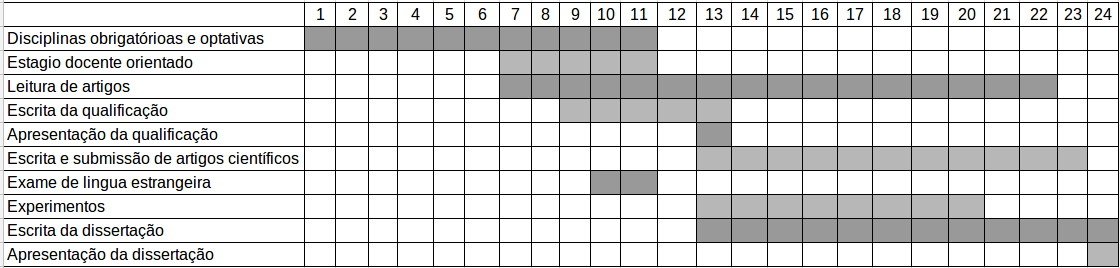
\includegraphics[width=1 \textwidth]{cronograma_atividades.png}
\begin{center}
\caption{Cronograma de atividades \label{cronograma_atividade}}
%Fonte: Elaborada pelo autor
\end{center}
\end{figure}




%%
%% Parte pos-textual
%%
\backmatter

% Apendices
% Comente se naoo houver apendices
\appendix

% Eh aconselhavel criar cada apendice em um arquivo separado, digamos
% "apendice1.tex", "apendice.tex", ... "apendiceM.tex" e depois
% inclui--los com:
\xchapter{Lista de Símbolos}{ }

\begin{tabular}{rl}
$[e_i,l_i]$ & Começo e fim de uma aç\~ ao envolvendo o indiv\'iduo $i$ \\
$d_p$ & Duraç\~ao do atendimento ao paciente $p$ \\
$\delta_{ij}$ & Medida de distância entre $i$ e $j$ \\
$\tau_{ij}$ & Medida de tempo entre os pontos $i$ e $j$ \\
$B$ & Conjunto de turnos \\
$D$ & Conjunto de dias \\
$E$ & Conjunto de enfermeiras \\
$L$ & Conjunto de pausas \\
$P$ & Conjunto de pacientes \\
$Q$ & Conjunto de clientes \\
$R$ & Conjunto de Restrições \\
$S$ & Conjunto de pessoas \\
$T$ & Conjunto de tarefas \\
$V$ & Conjunto de veículos \\
$W$ & Conjunto de locais \\
$X$ & Conjunto de variáveis \\
$\Omega$ & Conjunto de domínios \\
$\Omega\varepsilon$ & Relação das variáveis com os domínios 
\end{tabular}
% \include{apendice2}
% ...
% \include{apendiceM}

% Bibliografia
% BibTeXpress em www.cin.ufpe.br/~paguso/bibtexpress
\bibliographystyle{abntex2-alf}
\bibliography{biblio}

%% Fim do documento


\end{document}
